\documentclass{standalone}
\usepackage{tikz}
\usetikzlibrary{patterns, positioning}
\usepackage[sfdefault]{ClearSans} %% option 'sfdefault' activates Clear Sans as the default text font
\usepackage[T1]{fontenc}

\begin{document}
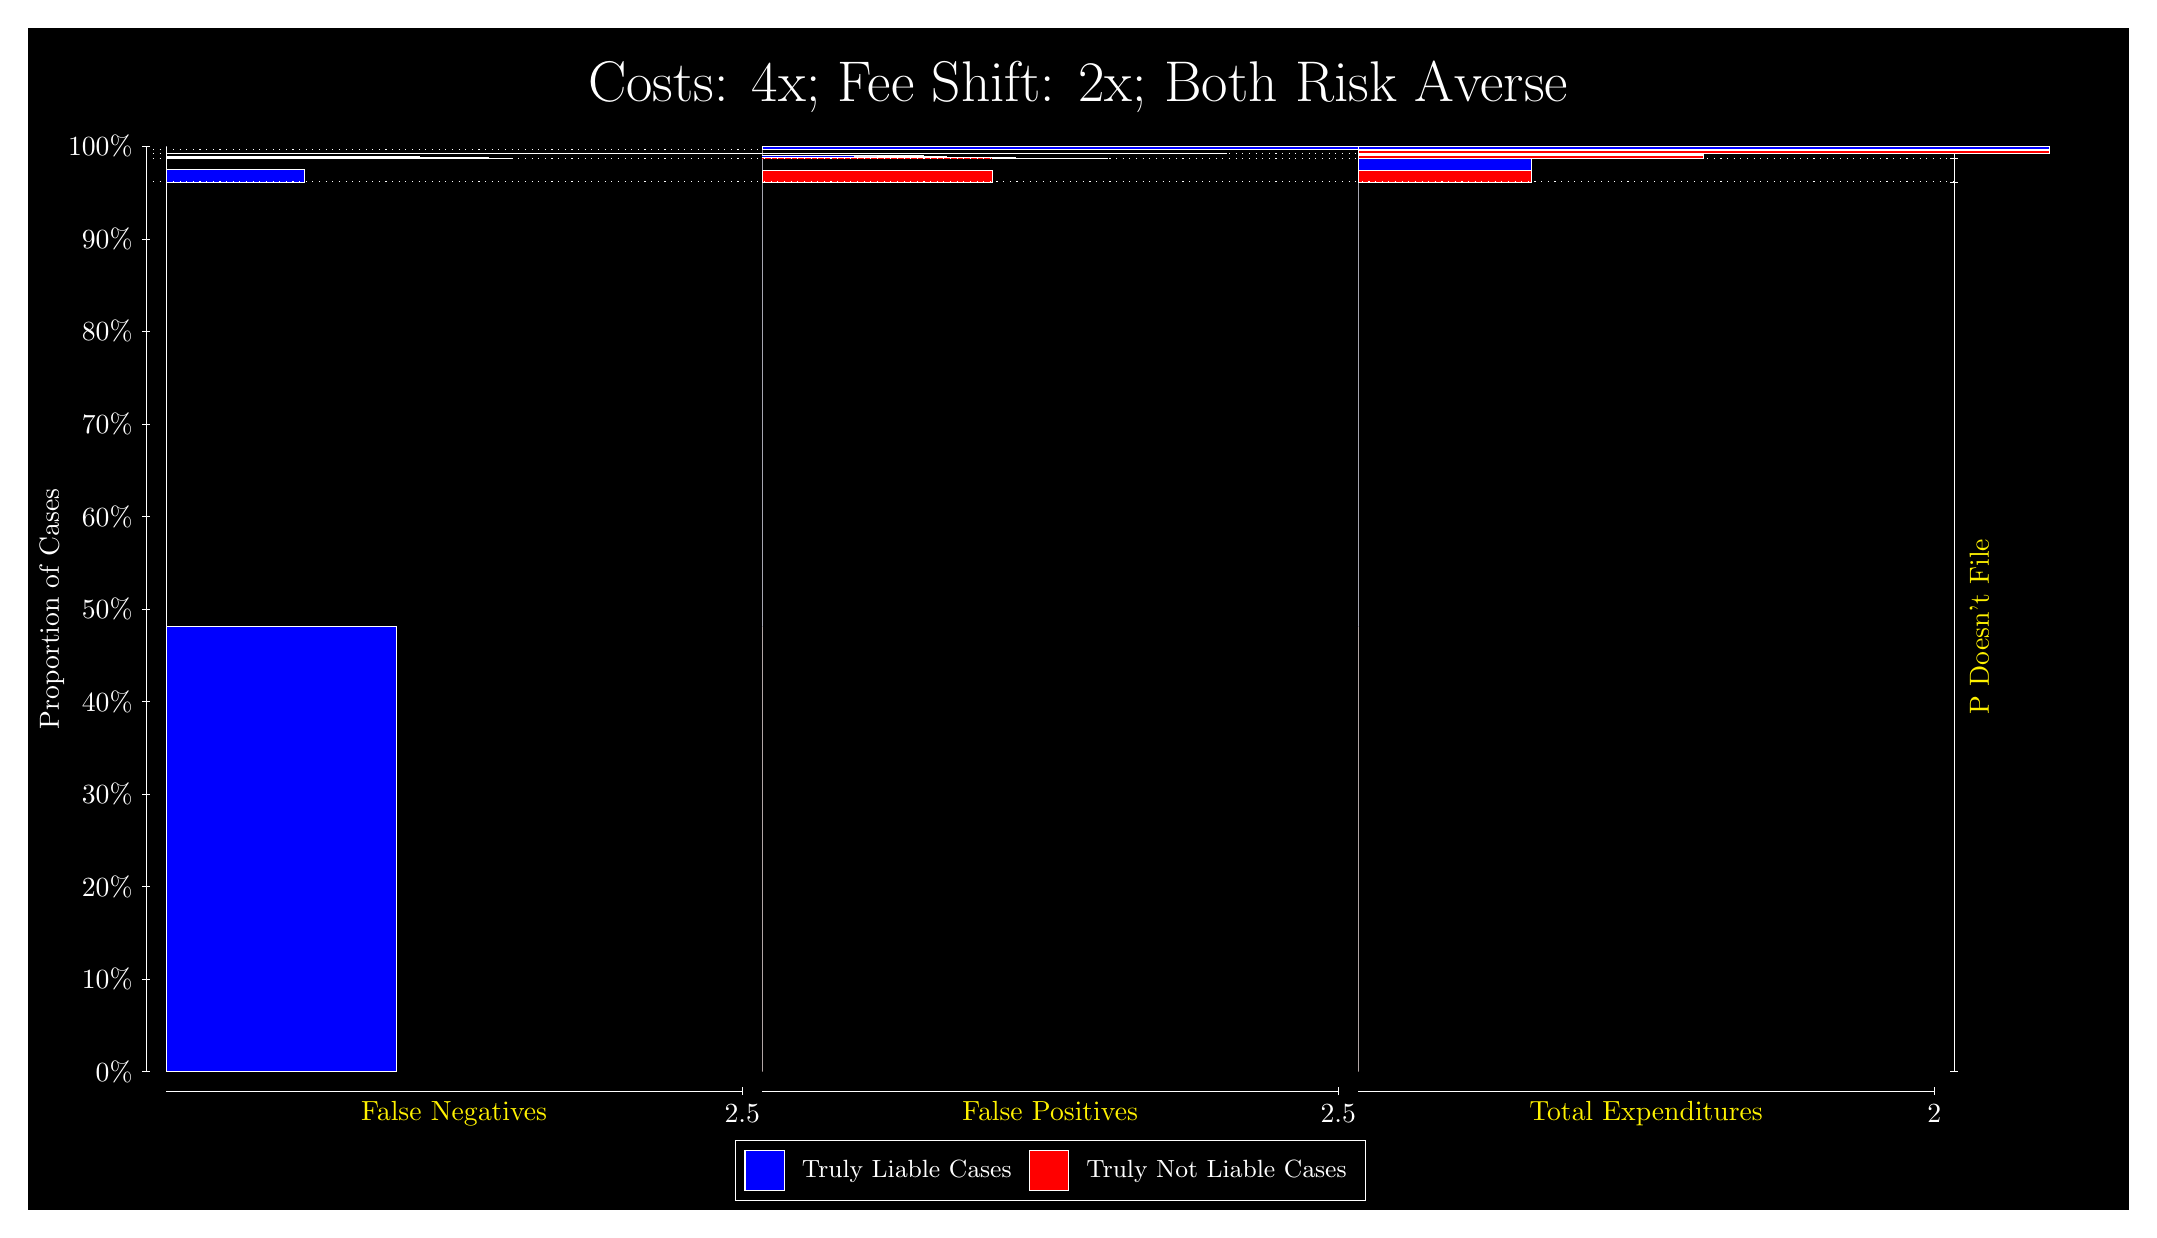
\begin{tikzpicture}
\draw[fill=black] (0,0) rectangle (26.667,15);
\draw[text=white] (0,13.5) rectangle (26.667,15) node[midway] {\huge Costs: 4x; Fee Shift: 2x; Both Risk Averse};
\draw[white, very thin] (1.5,1.75) -- (1.5,13.5);
\node[rotate=90, text=white, anchor=center] at (0.3, 7.625) {Proportion of Cases};
\draw[white, very thin] (1.45,1.75) -- (1.55,1.75);
\node[text=white, anchor=east] at (1.45, 1.75) {0\%};
\draw[white, very thin] (1.45,2.925) -- (1.55,2.925);
\node[text=white, anchor=east] at (1.45, 2.925) {10\%};
\draw[white, very thin] (1.45,4.1) -- (1.55,4.1);
\node[text=white, anchor=east] at (1.45, 4.1) {20\%};
\draw[white, very thin] (1.45,5.275) -- (1.55,5.275);
\node[text=white, anchor=east] at (1.45, 5.275) {30\%};
\draw[white, very thin] (1.45,6.45) -- (1.55,6.45);
\node[text=white, anchor=east] at (1.45, 6.45) {40\%};
\draw[white, very thin] (1.45,7.625) -- (1.55,7.625);
\node[text=white, anchor=east] at (1.45, 7.625) {50\%};
\draw[white, very thin] (1.45,8.8) -- (1.55,8.8);
\node[text=white, anchor=east] at (1.45, 8.8) {60\%};
\draw[white, very thin] (1.45,9.975) -- (1.55,9.975);
\node[text=white, anchor=east] at (1.45, 9.975) {70\%};
\draw[white, very thin] (1.45,11.15) -- (1.55,11.15);
\node[text=white, anchor=east] at (1.45, 11.15) {80\%};
\draw[white, very thin] (1.45,12.325) -- (1.55,12.325);
\node[text=white, anchor=east] at (1.45, 12.325) {90\%};
\draw[white, very thin] (1.45,13.5) -- (1.55,13.5);
\node[text=white, anchor=east] at (1.45, 13.5) {100\%};

\draw[white, very thin] (24.457,1.75) -- (24.457,13.5);
\draw[white, very thin] (24.407,1.75) -- (24.507,1.75);
\node[anchor=west] at (24.407, 1.75) {};
\draw[white, very thin] (24.407,13.049) -- (24.507,13.049);
\node[anchor=west] at (24.407, 13.049) {};
\draw[white, very thin] (24.407,13.345) -- (24.507,13.345);
\node[anchor=west] at (24.407, 13.345) {};
\draw[white, very thin] (24.407,13.409) -- (24.507,13.409);
\node[anchor=west] at (24.407, 13.409) {};
\draw[white, very thin] (24.407,13.458) -- (24.507,13.458);
\node[anchor=west] at (24.407, 13.458) {};
\draw[white, very thin] (24.407,13.5) -- (24.507,13.5);
\node[anchor=west] at (24.407, 13.5) {};

\draw[white, very thin, fill=blue] (1.75,1.75) rectangle (4.6775,7.3994);
\draw[white, very thin, fill=red] (1.75,7.3994) rectangle (1.75,13.049);
\draw[white, very thin, fill=blue] (1.75,13.049) rectangle (3.5065,13.203);
\draw[white, very thin, fill=red] (1.75,13.203) rectangle (1.75,13.345);
\draw[white, very thin, fill=blue] (1.75,13.345) rectangle (6.1413,13.35);
\draw[white, very thin, fill=blue] (1.75,13.35) rectangle (5.8486,13.357);
\draw[white, very thin, fill=blue] (1.75,13.357) rectangle (5.5558,13.365);
\draw[white, very thin, fill=blue] (1.75,13.365) rectangle (5.2631,13.367);
\draw[white, very thin, fill=blue] (1.75,13.367) rectangle (4.9703,13.37);
\draw[white, very thin, fill=blue] (1.75,13.37) rectangle (4.6775,13.372);
\draw[white, very thin, fill=blue] (1.75,13.372) rectangle (4.3848,13.373);
\draw[white, very thin, fill=blue] (1.75,13.373) rectangle (4.092,13.374);
\draw[white, very thin, fill=blue] (1.75,13.374) rectangle (3.7993,13.375);
\draw[white, very thin, fill=red] (1.75,13.375) rectangle (1.75,13.409);
\draw[white, very thin, fill=blue] (1.75,13.409) rectangle (15.217,13.418);
\draw[white, very thin, fill=red] (1.75,13.418) rectangle (1.75,13.458);
\draw[white, very thin, fill=red] (1.75,13.458) rectangle (1.75,13.467);
\draw[white, very thin, fill=blue] (1.75,13.467) rectangle (1.75,13.5);
\draw[white, very thin, fill=red] (9.3189,1.75) rectangle (9.3189,7.3995);
\draw[white, very thin, fill=blue] (9.3189,7.3995) rectangle (9.3189,13.049);
\draw[white, very thin, fill=red] (9.3189,13.049) rectangle (12.246,13.191);
\draw[white, very thin, fill=blue] (9.3189,13.191) rectangle (9.3189,13.345);
\draw[white, very thin, fill=red] (9.3189,13.345) rectangle (13.71,13.346);
\draw[white, very thin, fill=red] (9.3189,13.346) rectangle (13.417,13.347);
\draw[white, very thin, fill=red] (9.3189,13.347) rectangle (13.125,13.349);
\draw[white, very thin, fill=red] (9.3189,13.349) rectangle (12.832,13.351);
\draw[white, very thin, fill=red] (9.3189,13.351) rectangle (12.539,13.355);
\draw[white, very thin, fill=red] (9.3189,13.355) rectangle (12.246,13.358);
\draw[white, very thin, fill=red] (9.3189,13.358) rectangle (11.954,13.366);
\draw[white, very thin, fill=red] (9.3189,13.366) rectangle (11.661,13.373);
\draw[white, very thin, fill=red] (9.3189,13.373) rectangle (11.368,13.38);
\draw[white, very thin, fill=blue] (9.3189,13.38) rectangle (10.783,13.38);
\draw[white, very thin, fill=blue] (9.3189,13.38) rectangle (10.49,13.381);
\draw[white, very thin, fill=blue] (9.3189,13.381) rectangle (10.197,13.383);
\draw[white, very thin, fill=blue] (9.3189,13.383) rectangle (9.9044,13.384);
\draw[white, very thin, fill=blue] (9.3189,13.384) rectangle (9.6116,13.387);
\draw[white, very thin, fill=blue] (9.3189,13.387) rectangle (9.3189,13.409);
\draw[white, very thin, fill=red] (9.3189,13.409) rectangle (9.3189,13.449);
\draw[white, very thin, fill=blue] (9.3189,13.449) rectangle (9.3189,13.458);
\draw[white, very thin, fill=red] (9.3189,13.458) rectangle (22.786,13.467);
\draw[white, very thin, fill=blue] (9.3189,13.467) rectangle (19.858,13.5);
\draw[white, very thin, fill=red] (16.888,1.75) rectangle (16.888,7.3995);
\draw[white, very thin, fill=blue] (16.888,7.3995) rectangle (16.888,13.049);
\draw[white, very thin, fill=red] (16.888,13.049) rectangle (19.083,13.191);
\draw[white, very thin, fill=blue] (16.888,13.191) rectangle (19.083,13.345);
\draw[white, very thin, fill=red] (16.888,13.345) rectangle (21.279,13.349);
\draw[white, very thin, fill=blue] (16.888,13.349) rectangle (21.279,13.352);
\draw[white, very thin, fill=red] (16.888,13.352) rectangle (21.279,13.38);
\draw[white, very thin, fill=blue] (16.888,13.38) rectangle (21.279,13.404);
\draw[white, very thin, fill=red] (16.888,13.404) rectangle (21.279,13.407);
\draw[white, very thin, fill=blue] (16.888,13.407) rectangle (21.279,13.409);
\draw[white, very thin, fill=red] (16.888,13.409) rectangle (25.67,13.449);
\draw[white, very thin, fill=blue] (16.888,13.449) rectangle (25.67,13.458);
\draw[white, very thin, fill=red] (16.888,13.458) rectangle (25.67,13.467);
\draw[white, very thin, fill=blue] (16.888,13.467) rectangle (25.67,13.5);
\draw[white, dotted] (1.5,13.049) -- (24.457,13.049);
\draw[white, dotted] (1.5,13.345) -- (24.457,13.345);
\draw[white, dotted] (1.5,13.409) -- (24.457,13.409);
\draw[white, dotted] (1.5,13.458) -- (24.457,13.458);
\draw[white, very thin] (1.75,1.5) -- (9.0689,1.5);
\node[text=yellow, anchor=north] at (5.4094, 1.5) {False Negatives};
\draw[white, very thin] (9.0689,1.45) -- (9.0689,1.55);
\node[text=white, anchor=north] at (9.0689, 1.45) {2.5};

\draw[white, very thin] (9.3189,1.5) -- (16.638,1.5);
\node[text=yellow, anchor=north] at (12.978, 1.5) {False Positives};
\draw[white, very thin] (16.638,1.45) -- (16.638,1.55);
\node[text=white, anchor=north] at (16.638, 1.45) {2.5};

\draw[white, very thin] (16.888,1.5) -- (24.207,1.5);
\node[text=yellow, anchor=north] at (20.547, 1.5) {Total Expenditures};
\draw[white, very thin] (24.207,1.45) -- (24.207,1.55);
\node[text=white, anchor=north] at (24.207, 1.45) {2};

\node[text=yellow, centered, rotate=90] at (24.777, 7.3994) {P Doesn't File};





\draw (12.978300999999998,1.5) node[draw=none] (baseCoordinate) {};
\begin{scope}[align=center]
        \matrix[scale=0.5, draw=white, below=0.5cm of baseCoordinate, nodes={draw}, column sep=0.1cm]{
            \node[rectangle, draw, minimum width=0.5cm, minimum height=0.5cm, fill=blue] {}; &
            \node[draw=none, font=\small, text=white] (B) {Truly Liable Cases}; &
            \node[rectangle, draw, minimum width=0.5cm, minimum height=0.5cm, fill=red] {}; &
            \node[draw=none, font=\small, text=white] (B) {Truly Not Liable Cases}; \\
            };
\end{scope}

\end{tikzpicture}
\end{document}